% Resultados (consigna 2.2, ítem 8). Tablas y figuras importadas de ../salidas (generadas por codigo/04_analisis.py);
% cifras del texto desde generado/cifras.tex. Texto reescrito por el estudiante (26-nov-2026).
% Cada apartado: un párrafo con las cifras, la tabla y un recuadro con el resultado en una frase.
\section{Resultados}

\subsection{Verificación de la muestra}

En la Tabla~\ref{tab:muestra} se compara la cantidad de datos de cada variable con el mínimo requerido. Las series de tiempo tienen \cifra{muSeriesObs} meses por variable (\cifra{muSeriesDatos} datos, cuando se exigen \cifra{muSeriesMin}), el logit usa \cifra{muProyObs} proyectos y la comparación de rentabilidad, \cifra{muCompObs} empresas-trimestre o más. Si se toman solo los estados financieros de las plataformas, hay \cifra{muFpfObs} trimestres por variable, una cantidad que no llega al mínimo. Por eso esos datos solo se usan para describir, y la inferencia se hace con todas las empresas supervisadas.

\begin{table*}[!t]
\caption{Comprobación del tamaño de la muestra de cada variable}
\label{tab:muestra}
\small
\input{\tablas/t9_verificacion_muestra.tex}
\notaapa{Se cuentan los datos válidos (sin faltantes) de la variable con menos datos de cada bloque. obs. = observaciones. El último bloque tiene solo fines descriptivos. Elaboración propia con datos de la SMV \parencite{smvsimv2026,smvodata2026} y del BCRP \parencite{bcrpdata2026}.}
\end{table*}

\resultado{Cada variable incluida en un modelo alcanza el mínimo de 1\,000 observaciones o 60 periodos.}

\subsection{Evolución y estructura de la oferta}

Solo \cifra{plataformasConFinanciamiento} de las \cifra{plataformasAutorizadas} sociedades administradoras financiaron proyectos (Tabla~\ref{tab:plataformas} del Anexo). \cifra{nombreLider} financió \cifra{proyFinLider} proyectos por S/~\cifra{montoLider} millones, el \cifra{participacionLider}~\% del total. Entre 2022 y 2025, el monto anual subió de S/~\cifra{monto2022} millones a S/~\cifra{monto2025} millones (Tabla~\ref{tab:anual} y Figura~\ref{fig:monto}), y de enero a septiembre de 2026 llegó a S/~\cifra{monto2026} millones, un \cifra{varMonto2026}~\% más que en los mismos meses de 2025. El crecimiento se explica sobre todo por proyectos más grandes, ya que el monto medio pasó de S/~\cifra{montoMedio2022} mil en 2022 a S/~\cifra{montoMedio2026} mil en 2026. El índice de Herfindahl-Hirschman, que era de \cifra{hhi2022} en 2022, llegó a \cifra{hhi2025} en 2025.

\begin{table*}[!t]
\caption{Oferta anual de financiamiento participativo financiero, 2022-2026}
\label{tab:anual}
\small
\input{\tablas/t2_oferta_anual.tex}
\notaapa{La variación de 2026 compara enero-septiembre con los mismos meses de 2025. Los montos están en soles corrientes; los agregados excluyen los meses no obtenidos, por lo que son una cota inferior. Elaboración propia con datos de la \textcite{smvsimv2026}.}
\end{table*}

\begin{figure*}[!t]
\caption{Monto financiado mensual mediante plataformas de financiamiento participativo financiero, por plataforma (S/ millones corrientes)}
\label{fig:monto}
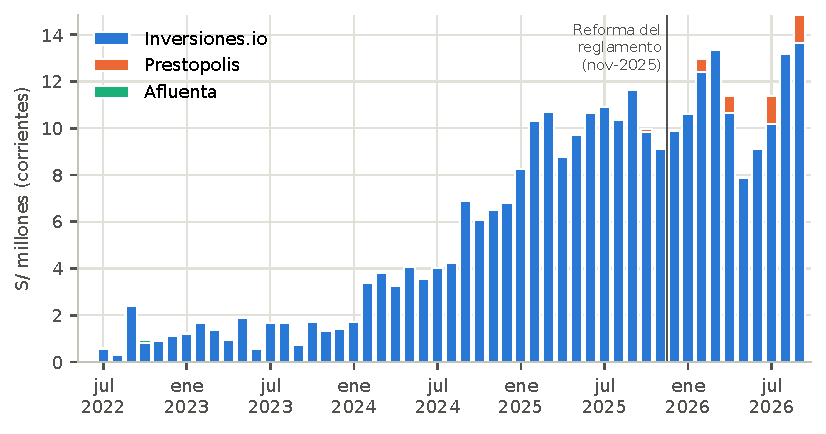
\includegraphics[width=0.78\linewidth]{f1_monto_mensual_por_plataforma.pdf}
\notaapa{La línea vertical marca diciembre de 2025, primer mes completo tras la modificación del reglamento. Elaboración propia con datos de la \textcite{smvsimv2026}.}
\end{figure*}

\resultado{El FPF se expandió rápido, aunque casi todo el monto se concentra en una sola plataforma.}

\subsection{Rentabilidad de las administradoras}

Entre las plataformas que financiaron proyectos, solo \cifra{nombreLider} tiene utilidades, desde \cifra{primerAnioUtilidadLider}, con un ROA de \cifra{roaLider2025}~\% en 2025, y sus ingresos equivalen, en la mediana, al \cifra{costoMediana}~\% del monto que financia (Tabla~\ref{tab:financieros} del Anexo). El ROA trimestral mediano de las plataformas es \cifra{empRoaMedFpf}~\%, mientras que el de los demás intermediarios es \cifra{empRoaMedResto}~\%. Cuando se controla por tamaño y trimestre, la diferencia es de \cifra{empRoa} puntos y no resulta significativa ($p\cifra{empRoaPRel}$), y tampoco lo es frente al total de empresas ($p\cifra{empRoaTodasPRel}$; Tabla~\ref{tab:rentabilidad}). En cambio, el tamaño sí se asocia con una mayor rentabilidad (\cifra{empRoaTam}; $p\cifra{empRoaTamPRel}$).

\begin{table*}[!t]
\caption{Rentabilidad y capital de las plataformas comparados con los de otras empresas supervisadas por la SMV}
\label{tab:rentabilidad}
\small
\input{\tablas/t15_rentabilidad_empresas.tex}
\notaapa{Estimación por mínimos cuadrados con efectos de trimestre (que no se muestran) y errores agrupados por empresa. El ROA y el patrimonio/activo están en porcentaje y acotados a los percentiles 1 y 99. Como solo hay cinco plataformas, la prueba tiene baja potencia. Elaboración propia con datos de la API OData de la SMV \parencite{smvodata2026}.}
\end{table*}

\resultado{En la mediana, las plataformas son menos rentables que los demás intermediarios, pero la brecha deja de ser significativa cuando se controla el tamaño.}

\subsection{Condiciones del crédito tradicional}

El crédito tradicional tiene tasas altas y muy distintas entre segmentos (Figura~\ref{fig:tasas} y Tabla~\ref{tab:segmentos} del Anexo). De 2022 a 2026, la TEA bancaria a pequeña y microempresa de hasta 360 días subió de \cifra{teaBcosPyme2022}~\% a \cifra{teaBcosPyme2026}~\%, y la de consumo, de \cifra{teaBcosConsumo2022}~\% a \cifra{teaBcosConsumo2026}~\%. En las cajas municipales, la tasa a pequeña y microempresa se mantuvo entre \cifra{teaCmacPymeMin}~\% y \cifra{teaCmacPymeMax}~\%, y en las rurales, entre \cifra{teaCracPymeMin}~\% y \cifra{teaCracPymeMax}~\%.

\begin{figure*}[!t]
\caption{Tasas activas promedio del crédito tradicional en moneda nacional por segmento}
\label{fig:tasas}
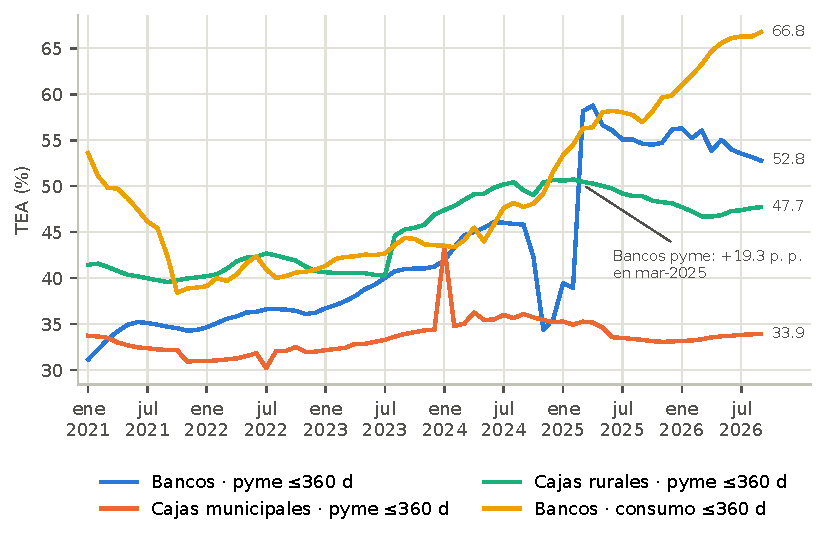
\includegraphics[width=0.78\linewidth]{f3_tasas_credito_tradicional.pdf}
\notaapa{Tasas efectivas anuales de préstamos de hasta 360 días. Elaboración propia con datos de \textcite{bcrpdata2026}.}
\end{figure*}

\resultado{En promedio anual, el crédito tradicional comparable cuesta como mínimo \cifra{teaCmacPymeMin}~\%. El FPF no tiene una tasa publicada con la que se pueda comparar.}

\subsection{Estacionariedad}

La prueba ADF no rechaza la raíz unitaria en niveles para ninguna de las \cifra{raizN} series, pero sí la rechaza en todas cuando se toman primeras diferencias (Tabla~\ref{tab:raiz}). En el caso del monto del FPF, el valor $p$ pasa de $p\cifra{adfFpfPRel}$ a $p\cifra{adfFpfDifPRel}$. La KPSS respalda este resultado, excepto en la tasa de consumo y en el IPC, que se toman con reserva. Según la prueba de Zivot-Andrews, \cifra{zaQuiebres} tasas son estacionarias en torno a un quiebre, entre ellas la de los bancos a pymes (\cifra{zaBancosMes}).

\begin{table*}[!t]
\caption{Resultados de las pruebas de raíz unitaria (69 meses)}
\label{tab:raiz}
\footnotesize
\input{\tablas/t10_raiz_unitaria.tex}
\notaapa{ADF y KPSS se estiman con constante, y los valores $p$ de la KPSS están acotados a [0.01; 0.10]. Zivot-Andrews se estima con cambio de nivel; entre paréntesis figura el primer mes del nuevo nivel. Elaboración propia con datos de la \textcite{smvsimv2026} y de \textcite{bcrpdata2026}.}
\end{table*}

\resultado{De acuerdo con la ADF, las series son integradas de orden uno, por lo que corresponde probar la cointegración y, si no existe, trabajar con las diferencias.}

\subsection{Relación de largo plazo}

Con 69 meses, la prueba de Engle-Granger no rechaza la ausencia de cointegración en ninguno de los pares (el valor $p$ más bajo es \cifra{egParesPMin}) ni en el sistema de cuatro tasas ($p\cifra{egSistemaPRel}$). La traza de Johansen tampoco supera su valor crítico: en el par más cercano llega a \cifra{johParesMax} frente a \cifra{johBancosVC}, y en el sistema, a \cifra{johSistema} frente a \cifra{johSistemaVC} (Tabla~\ref{tab:cointegracion}). Ninguna de las pruebas de Granger resulta significativa (el menor $p$ es \cifra{grangerPMin}). Si se usan solo los \cifra{mesesActividadFPF} meses con actividad, Engle-Granger sí rechaza con la tasa de los bancos a pymes ($p\cifra{egBancosActivosPRel}$) y con el sistema ($p\cifra{egSistemaActivosPRel}$), así que la conclusión cambia según la muestra.

\begin{table*}[!t]
\caption{Resultados de cointegración y causalidad de Granger (69 meses)}
\label{tab:cointegracion}
\footnotesize
\input{\tablas/t11_cointegracion.tex}
\notaapa{La hipótesis nula es que no existe cointegración. En Johansen se usa la traza para $r=0$ con constante, y Granger se estima en primeras diferencias con un rezago. La columna de 52 meses es un análisis de sensibilidad con menos de 60 periodos. Elaboración propia con datos de la \textcite{smvsimv2026} y de \textcite{bcrpdata2026}.}
\end{table*}

\resultado{No se encuentra evidencia sólida de que el monto del FPF y las tasas del crédito tradicional mantengan una relación estable de largo plazo.}

\subsection{Relación de corto plazo}

Cuando el modelo incluye variables de impulso, ninguna tasa es significativa, ni por separado ni en conjunto ($p\cifra{cpConWaldPRel}$; Tabla~\ref{tab:corto}). Si se quitan los impulsos, la tasa de las cajas municipales aparece como significativa ($p\cifra{cpSinCmacPRel}$), pero eso se debe a un único salto que se revierte al mes siguiente. El único efecto estable es el del propio rezago ($\varphi=\cifra{cpConPhi}$, $p\cifra{cpConPhiPRel}$), lo que indica que a un mes alto suele seguirle uno más bajo. Los diagnósticos no muestran autocorrelación, heterocedasticidad, mala especificación ni inestabilidad. Los residuos no siguen una distribución normal ($p\cifra{cpConJbPRel}$), así que la inferencia es asintótica. Si se usan solo los meses de actividad, las tasas son significativas en conjunto ($p\cifra{cpActivosWaldPRel}$), aunque ninguna lo es individualmente.

\begin{table*}[!t]
\caption{Modelo de corto plazo del monto del FPF estimado con errores HAC}
\label{tab:corto}
\footnotesize\tablacompacta
\input{\tablas/t12_corto_plazo_hac.tex}
\notaapa{La variable dependiente es la primera diferencia del asinh del monto mensual, en millones de soles de diciembre de 2021. Los valores $p$ se calculan con errores HAC. Cada impulso vale uno en un único mes. Elaboración propia con datos de la \textcite{smvsimv2026} y de \textcite{bcrpdata2026}.}
\end{table*}

\resultado{Con los 67 cambios mensuales disponibles, las variaciones de las tasas tradicionales no explican las del monto del FPF en el corto plazo.}

\subsection{Modificación del reglamento (H1)}

La mediana mensual subió de S/~\cifra{hUnoMedianaAntes} millones antes de la modificación a S/~\cifra{hUnoMedianaDespues} millones después ($U=\cifra{hUnoU}$, $p\cifra{hUnoPRel}$), aunque esta comparación no toma en cuenta la tendencia. Si se descuenta, el nivel y la pendiente posteriores quedan por debajo de lo que proyectaba la tendencia previa en escala asinh (\cifra{refAsinhNivel}, $p\cifra{refAsinhNivelPRel}$; \cifra{refAsinhPend}, $p\cifra{refAsinhPendPRel}$). Con errores AR(1), ninguno de los dos coeficientes es significativo por separado, pero sí lo son en conjunto ($p\cifra{refArWaldPRel}$), y con el monto en millones de soles no hay cambio ($p\cifra{refLinWaldPRel}$; Tabla~\ref{tab:reforma} y Figura~\ref{fig:reforma}). Incluso \cifra{refPlacebos} de los \cifra{refPlacebosN} cortes ficticios anteriores resultan significativos.

\begin{table*}[!t]
\caption{Regresión segmentada del monto mensual alrededor de la modificación del reglamento}
\label{tab:reforma}
\small
\input{\tablas/t13_reforma_segmentada.tex}
\notaapa{En los modelos (1) y (2) se usa el asinh del monto en millones de soles de diciembre de 2021, y en el (3), el monto sin transformar. MCG AR(1) significa mínimos cuadrados generalizados con errores autorregresivos. Elaboración propia con datos de la \textcite{smvsimv2026} y de \textcite{bcrpdata2026}.}
\end{table*}

\begin{figure*}[!t]
\caption{Monto mensual financiado y regresión segmentada alrededor de la modificación del reglamento}
\label{fig:reforma}
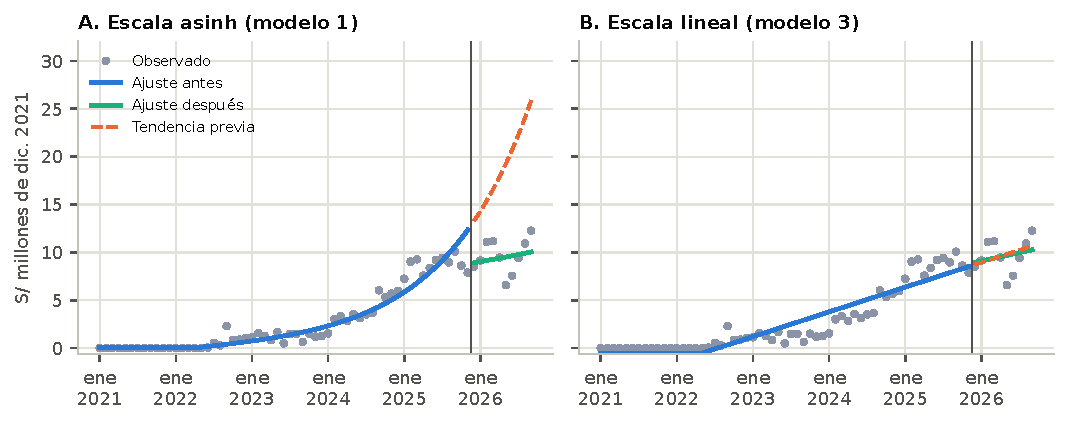
\includegraphics[width=0.86\linewidth]{f5_reforma_segmentada.pdf}
\notaapa{La línea discontinua extiende la tendencia que había antes de diciembre de 2025. Elaboración propia con datos de la \textcite{smvsimv2026} y de \textcite{bcrpdata2026}.}
\end{figure*}

\resultado{H1 solo se cumple al describir los niveles. No hay evidencia de que la modificación del reglamento haya tenido un efecto positivo.}

\subsection{Acceso por tipo de receptor (H2)}

De los \cifra{publicadosEmp} proyectos empresariales se financió el \cifra{colocacionEmp}~\%, y de los \cifra{publicadosPer} personales, el \cifra{colocacionPer}~\% (Tabla~\ref{tab:condiciones} del Anexo). Según el logit, un proyecto empresarial tiene una razón de momios de \cifra{logUnoOr} ($p\cifra{logUnoPRel}$), lo que equivale a un efecto marginal de \cifra{logUnoEfecto} puntos porcentuales. Cuando se controla por plataforma y año, la razón baja a \cifra{logTresOr} (IC 95~\% [\cifra{logTresInf}; \cifra{logTresSup}], $p\cifra{logTresPRel}$), con un efecto de \cifra{logTresEfecto} puntos y un intervalo que casi toca el cero (Tabla~\ref{tab:logit}). Hay que tomar esto con cautela, porque el \cifra{pctEmpresarialPrincipal}~\% de los proyectos empresariales corresponde a \cifra{nombreLider} y el \cifra{pctPersonalPrincipal}~\% de los personales, a \cifra{principalPersonal}. Dentro de \cifra{nombreLider}, la prueba exacta de Fisher no resulta significativa ($p\cifra{hDosFisherPRel}$). La colocación también mejora con los años (\cifra{logAnioOr}; $p\cifra{logAnioPRel}$).

\begin{table*}[!t]
\caption{Logit de la probabilidad de colocación de los proyectos publicados}
\label{tab:logit}
\small
\input{\tablas/t14_logit_colocacion.tex}
\notaapa{Se reportan razones de momios con intervalos de confianza al 95~\%. El efecto marginal corresponde al promedio de la muestra. Se asume que los proyectos son independientes. Elaboración propia con datos de la \textcite{smvsimv2026}.}
\end{table*}

\resultado{Los proyectos empresariales logran colocarse más, aunque gran parte de esa ventaja se explica por la plataforma y el año.}
